\subsection{�bertragungsfunktion des geschlossenen Regelkreises}\label{StepResponse}

Die Berechnung des geschlossenen Regelkreises erfolgt mittels der �bertragungsfunktionen der Strecke (Formel \ref{eq:�bertragungsfunktionStrecke}) und der des Reglers (Formel \ref{eq:PITransmit} und \ref{eq:PIDTransmit}):

\begin{equation}
G(s)=\frac{G_{R}(s)\cdot G_{S}(s)}{1+G_{R}(s)\cdot G_{S}(s)}
\label{eq:GsStepResponse}
\end{equation}


Die Funktionen $G_{R}(s)$ und $G_{S}(s)$ werden nun in $B_{R}(s)$, $A_{R}(s)$, $B_{S}(s)$, $A_{S}(s)$ aufgeteilt, wobei $B_{R}(s)$ und $A_{R}(s)$ das Z�hler- bzw. das Nennerpolynom von $G_{R}(s)$ ist. Analog sind $B_{S}(s)$ und $A_{S}(s)$ die jeweiligen Polynome von $G_{S}(s)$.\\


Eingesetzt in die Formel \ref{eq:GsStepResponse} ergibt dies folgende Gleichung:

\begin{equation}
G(s)=\frac{\frac{B_{R}(s)\cdot B_{S}(s)}{A_{R}(s)\cdot A_{S}(s)}}{1+\frac{B_{R}(s)\cdot B_{S}(s)}{A_{R}(s)\cdot A_{S}(s)}}
\label{eq:GsStepAB}
\end{equation}

Ausmultipliziert erhalten wir:

\begin{equation}
G(s)=\frac{B_{R}(s)\cdot B_{S}(s)}{A_{R}(s)\cdot A_{S}(s)+B_{R}(s)\cdot B_{S}(s)}
\label{eq:GsStepABshort}
\end{equation}

Nun setzen wir $B_{R}(s)\cdot B_{S}(s)$ mit $B(s)$ und $A_{R}(s)\cdot A_{S}(s)$ mit $A(s)$ gleich, welches folgendes Resultat ergibt:

\begin{equation}
G(s)=\frac{B(s)}{A(s)}
\label{eq:ABstep}
\end{equation}

\textbf{Polynom-Bestimmung beim PI-Regler}

Als Grundlage werden die �bertragungsfunktionen der Strecke und die des PI-Reglers genommen (Formeln \ref{eq:�bertragungsfunktionStrecke} und \ref{eq:PITransmit}). Dabei wird angenommen, dass die Strecke erster Ordnung sei.

F�r die Strecke kann aus dem Z�hlerpolynom 0 herausgelesen werden. Das Nennerpolynom besteht aus den Koeffizienten $Ti$ und 0. Eingesetzt ergibt das:

\[
B_{S}(s)= 
\begin{bmatrix}
0
\end{bmatrix}
\]

\[
A_{S}(s)=
\begin{bmatrix}
Ti & 0
\end{bmatrix}
\]

Die Funktion der Strecke muss umgeformt werden:

\[
G_{R}(s)=\frac{s\cdot Tn\cdot Kr+Kr}{s\cdot Tn}
\]

\newpage
Daraus k�nnen wiederum $B_{R}(s)$ und $A_{R}(s)$ bestimmt werden:

\[
B_{R}(s)= 
\begin{bmatrix}
Tn\cdot Kr & Kr
\end{bmatrix}
\]

\[
A_{R}(s)=
\begin{bmatrix}
Tn
\end{bmatrix}
\]

\textbf{Polynom-Bestimmung beim PID-Regler}

Als Regelstrecke wird wiederum eine Strecke 1. Ordnung verwendet, woraus sich direkt die Koeffizienten der Streckenpolynome bestimmen lassen:


\[
B_{S}(s)= 
\begin{bmatrix}
0
\end{bmatrix}
\]

\[
A_{S}(s)=
\begin{bmatrix}
Ti & 0
\end{bmatrix}
\]

Die Formel \ref{eq:PIDTransmit} muss zuerst noch umgeformt werden:

\[
G_{R}(s)=\frac{s^{2}\cdot\left(Kr\cdot Tp \cdot Tn+Kr\cdot Tn\cdot Tv\right)+s\cdot\left(Kr\cdot Tn+Kr\cdot Tp\right)+Kr}{s^{2}\cdot\left(Tp\cdot Tn\right)+s\cdot Tn}
\]

Folgende Koeffizienten k�nnen herausgelesen werden:

\[
B_{R}(s)= 
\begin{bmatrix}
Kr\cdot Tp \cdot Tn+Kr\cdot Tn\cdot Tv & Kr\cdot Tn+Kr\cdot Tp & Kr
\end{bmatrix}
\]

\[
A_{R}(s)=
\begin{bmatrix}
Tp\cdot Tn & Tn
\end{bmatrix}
\]

\subsubsection{Berechnungsarten}

Zur weiteren Berechnung der Schrittantwort wurden folgende Methoden verwendet: IFFT (Inverse Fast Fourier Transformation) und Residuenberechnung (Partialbruchzerlegung).

\textbf{IFFT}

Zuerst wird bei der IFFT der Frequenzgang berechnet. Aus diesem kann die Impulsantwort berechnet werden. Die Werte der Impulsantwort aufsummiert ergeben die Schrittantwort.

\textbf{Residuen}

Als erstes werden die f�hrenden Nullstellen von $A(s)$ und $B(s)$ entfernt. Danach bestimmt man die Ordnung der Z�hler- und Nennerpolynome. Falls diese die gleiche Ordnung haben, muss zuerst eine Polynomdivision durchgef�hrt werden, um die Konstante $K$ zu bestimmen. 
Nun werden die Nullstellen von $A(s)$ und $B(s)$ berechnet, worauf die Residuen bestimmt werden k�nnen. 
Mittels dieser Residuen wird die Impulsantwort bestimmt. Aufsummiert ergibt diese die Schrittantwort.
\newpage
\textbf{Schrittantwort PI-Regler}

F�r die Simulation der Schrittantwort eines PI-Reglers werden wieder genau die gleichen Werte verwendet wie beim Beispiel in Kapitel \ref{PIExample}:

$Ks$ = 0.5\\
$Tu$ = 2.5\\
$Tg$ = 18.3\\
$\phi_{Strecke}$ = -114.6\textdegree (entspricht 4,6\% �berschwingen)\\
$Tn = 7.0647s$\\
$Kr = 0.9625$\\

\begin{figure}[h]	
	\centering		
	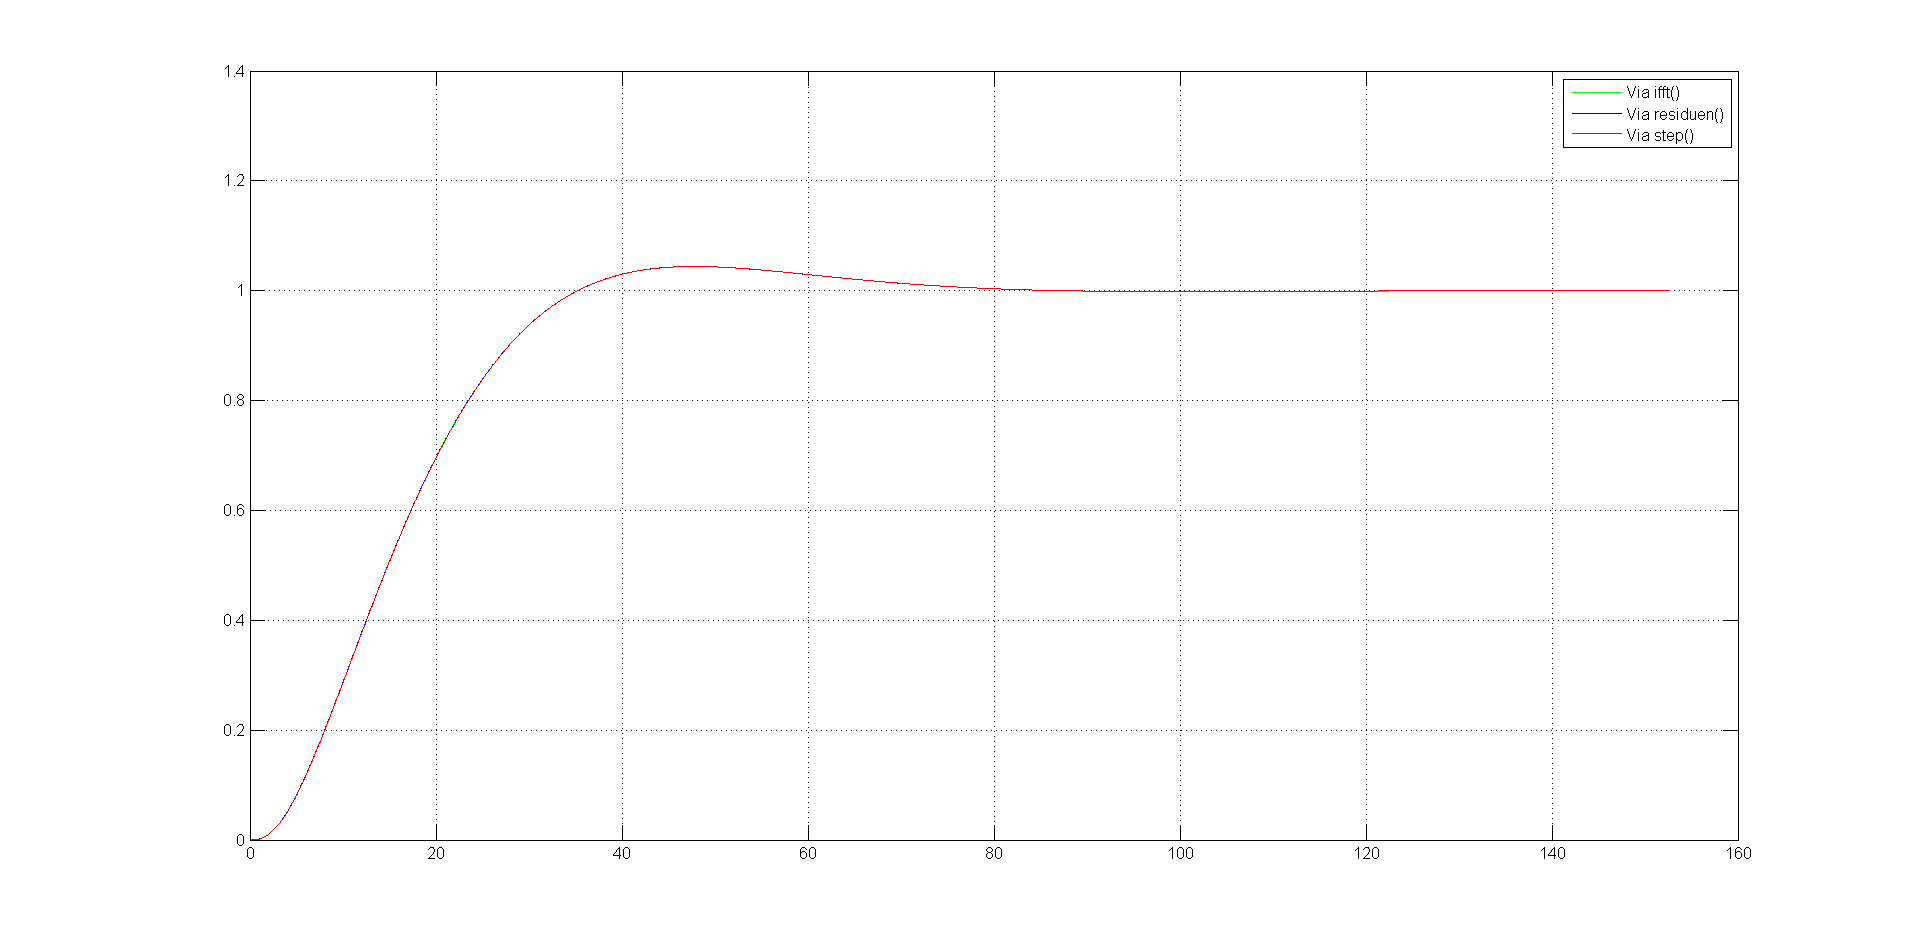
\includegraphics[width=1.0\textwidth]{PI_StepResponse.png}
	\caption{Simulation Schrittantwort}	
	\label{fig:PI_StepResponse}	
\end{figure}

\newpage
Als Vergleich wurde die step() Funktion von Matlab verwendet. Abweichungen sind fast nicht zu erkennen, erst wenn man die Abbildung vergr�ssert sind kleine Unterschiede festzustellen:

\begin{figure}[h]	
	\centering		
	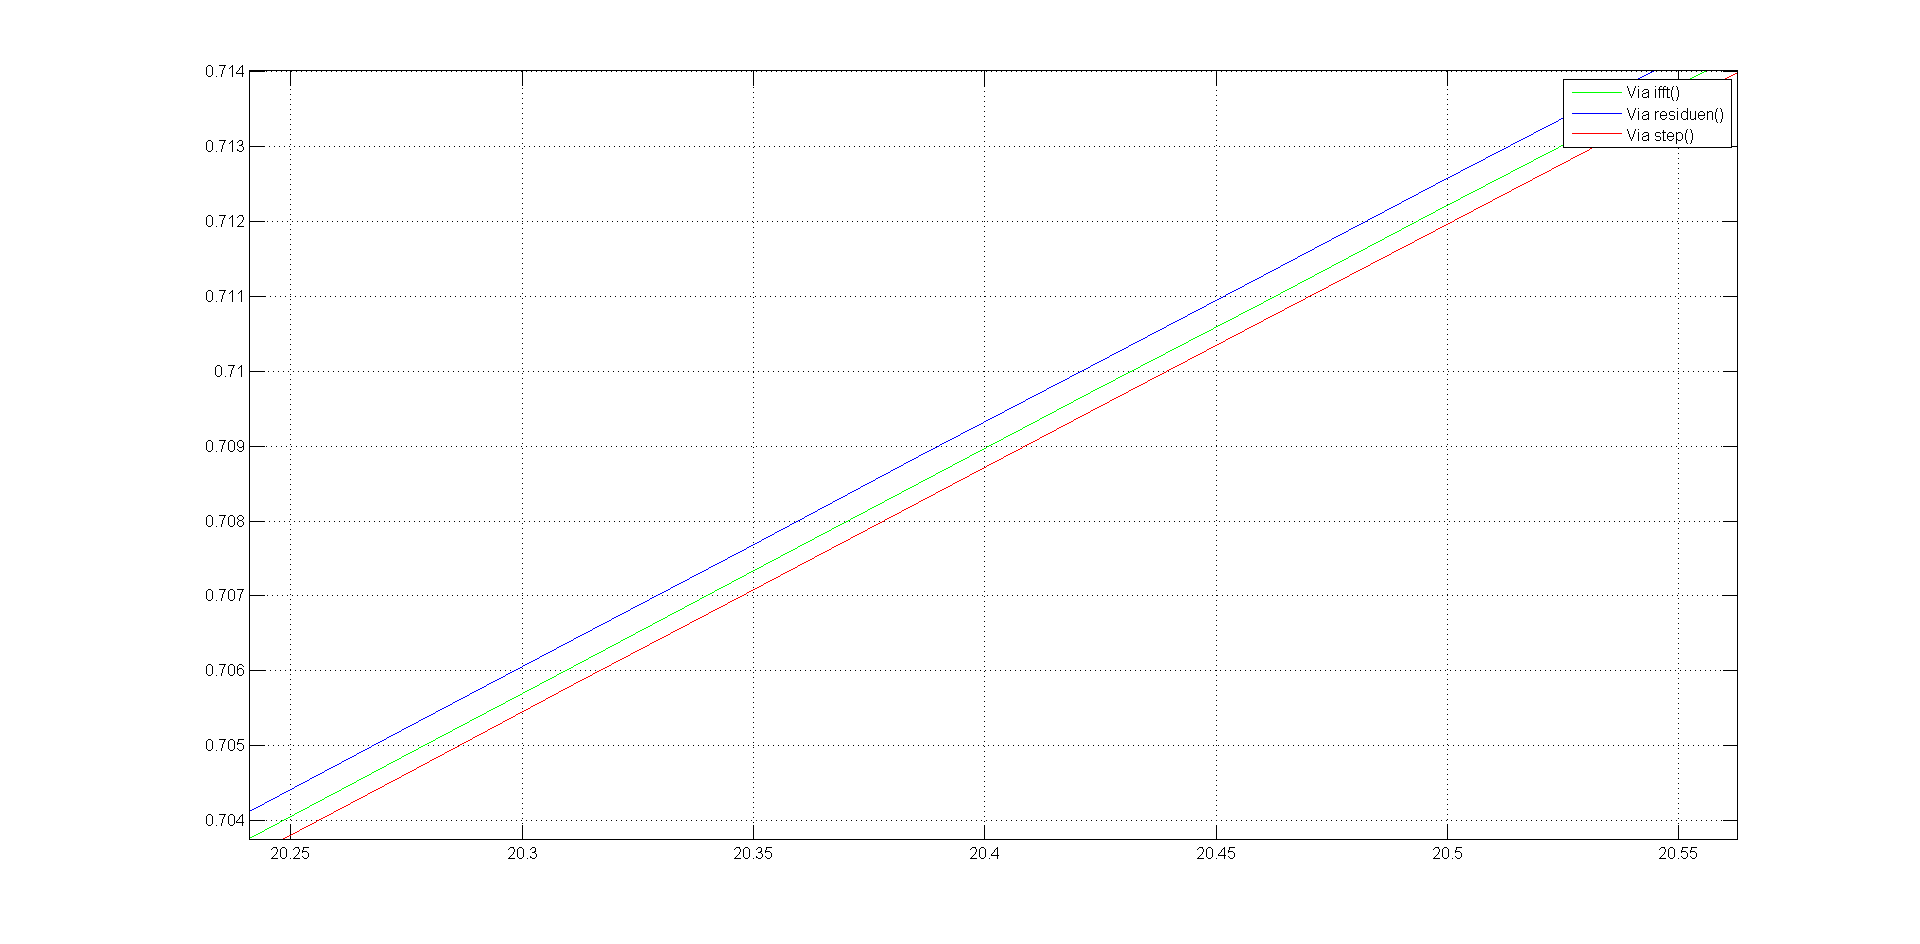
\includegraphics[width=1.0\textwidth]{PI_Step_Difference.png}
	\caption{Abweichungen der Berechnungsarten}	
	\label{fig:PI_Step_Difference}	
\end{figure}

\newpage
\textbf{Schrittantwort PID-Regler}

F�r die Simulation der Schrittantwort eines PID-Reglers werden wiederum die gleichen Werte verwendet wie beim Beispiel in Kapitel \ref{PIDExample}:

$Ks=0.5$\\
$Tu=2.5$\\
$Tg=18.3$\\
$\phi_{Strecke}$=-114.6\textdegree\\
$Tn =11.4521$\\
$Tv =0.8721$\\
$Kr =3.2963$\\

\begin{figure}[h]	
	\centering		
	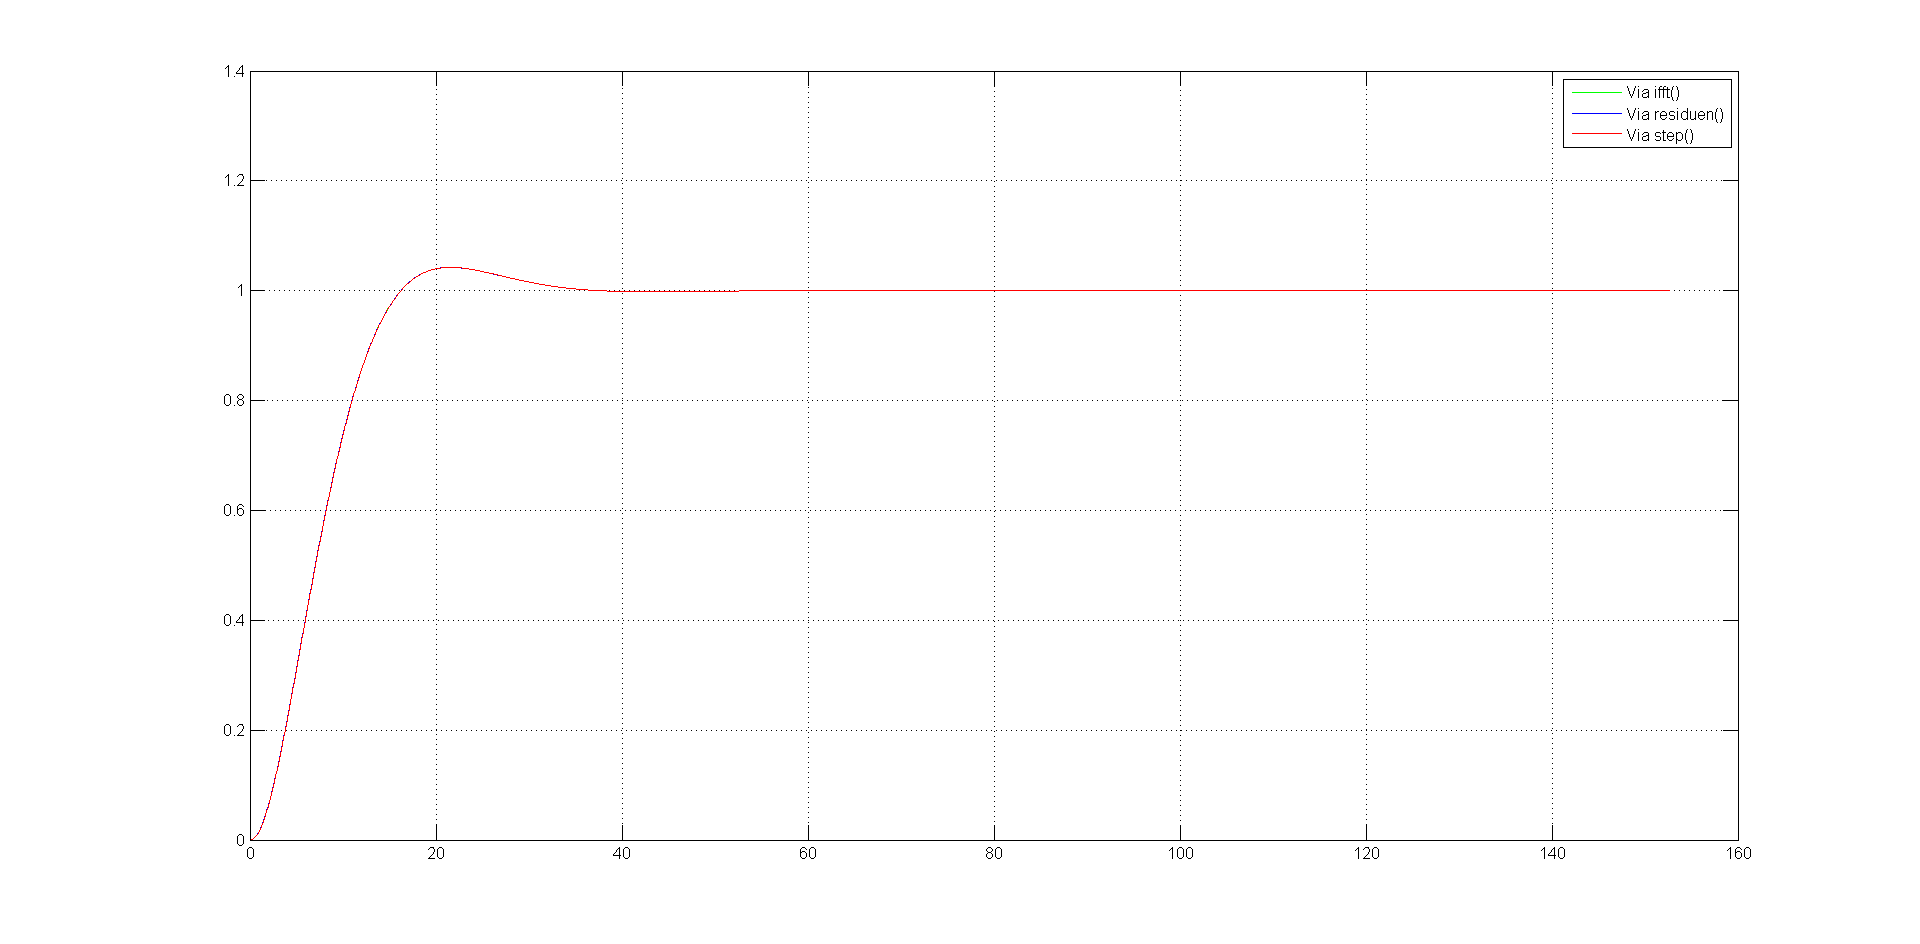
\includegraphics[width=1.0\textwidth]{PID_StepResponse.png}
	\caption{Simulation Schrittantwort}	
	\label{fig:PID_StepResponse}	
\end{figure}
\newpage
Als Vergleichswert wurde auch wieder die step() Funktion von Matlab verwendet. Um Abweichungen zu verdeutlichen, muss die Abbildung vergr�ssert werden:

\begin{figure}[h]	
	\centering		
	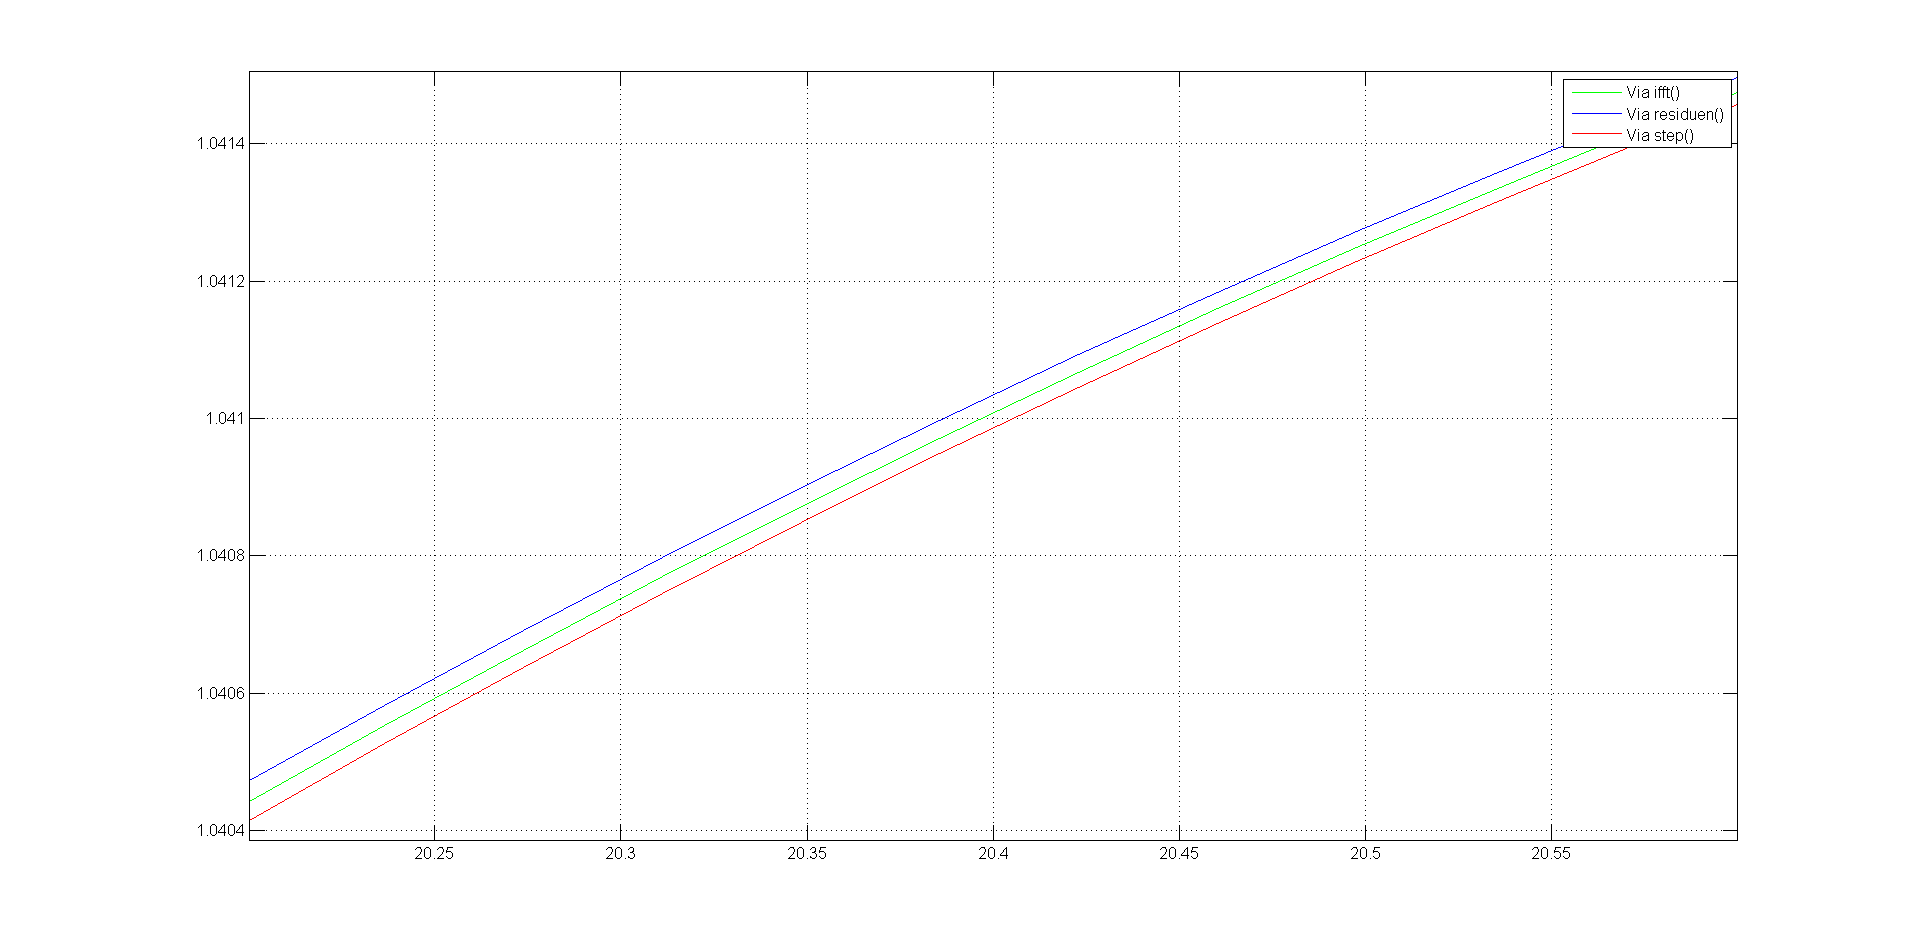
\includegraphics[width=1.0\textwidth]{PID_Step_Difference.png}
	\caption{Abweichungen der Berechnungsarten}	
	\label{fig:PID_Step_Difference}	
\end{figure}
